\chapter{Softwareentwurf}
Nach \cite{Balzert201109} ist der Softwareentwurf die Entwicklung einer software-technischen L�sung im Sinne einer Softwarearchitektur auf Basis der gegebenen Anforderungen an ein Softwareprodukt. 
Die Kunst bei einem Softwareentwurf besteht entsprechend darin, eine Softwarearchitektur zu entwerfen, die die zuvor erarbeiteten funktionalen (Kapitel \ref{sec:FunktionaleAnforderungen}) und nichtfunktionalen Anforderungen (Kapitel \ref{sec:NFA}) betrachtet, einschliesslich der Ber�cksichtigung von Einflussfaktoren wie definierte Randbedingungen. (Kaptitel \ref{sec:Randbedingungen}).
Der Softwareentwurf ist als Richtlinie zu sehen, der bei der Umsetzung der angeforderten Software unterst�tzt.
Die zu erstellende Softwarearchitektur hingegen beschreibt Architekturbausteine, deren Interaktionen und Beziehungen untereinander sowie ggf. deren Verteilung auf physicher Ebene. Dabei ist die spezifizierung der entsprechenden Schnittstellen der einzelnen Architekturbausteine mit zu beachten. F�r die Visualisierung der Architekturbausteine k�nnen verschiedene Abstufungen von Sichten herangezogen werden.
Die Kontextabgrenzung, Bausteinsicht, Laufzeitsicht und die Verteilungssicht.
\begin{comment}
\begin{enumerate}
\item \textbf{Kontextabgrenzung}
%Die Kontextabgrenzung beschreibt die Einbettung des Systems in seine Umgebung 
%sowie die wesentlichen Teile der umgebenden Infrastruktur.
\item \textbf{Bausteinsicht}
%Die Kontextabgrenzung beschreibt die Einbettung des Systems in seine Umgebung sowie die wesentlichen Teiler der umgebenden Infrastruktur.
\item \textbf{Laufzeitsicht}
\item \textbf{Verteilungssicht}
\end{enumerate}
\end{comment}
\begin{figure}[htbp]
  \centering
  \fbox{
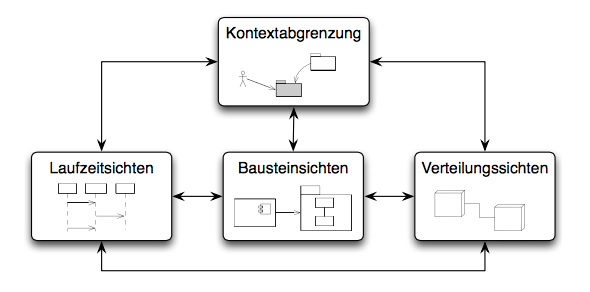
\includegraphics[width=0.9\textwidth]{../Bilder/sichten.png}
  }
  \caption{Vier Arten von Sichten (\cite{Starke201401})}

\end{figure}
\FloatBarrier

\section{Kontextabgrenzung}
Die Kontextabgrenzung beschreibt die Einbettung des Systems in seine Umgebung sowie die wesentlichen Teile der umgebenden Infrastruktur.
Die ermittelten Anforderungen aus Kapitel \ref{sec:FunktionaleAnforderungen} und \ref{NFA} haben ergeben, dass die Hauptfunktionalit�ten aus erstellen, exportieren, importieren, teilen und dem Provisioning von virtuellen Maschinen bestehen.
Um dies weiter zu b�ndeln, k�nnen Teile der Hauptfunktionali�ten von bestimmten Produkten �bernommen werden. 
Frei erh�ltliche Virtualisierungsprodukte k�nnen das Erstellen, Exportieren und den Import von virtuellen Maschinen �bernehmen. Software-Provisioner sind meist darauf ausgelegt, mit bekannten Virtualisierungsl�sungen zusammen zu arbeiten und �bernehmen somit die gew�nschten Anforderung nach automatisierter Softwareinstallation.
Der Kern der Anwendung organisiert das zusammenspiel der einzelnen Softwareprodukte und stellt dem Anwender die entsprechende Benutzeroberfl�che zur Verf�gung.
Die Anwendung selbst, inklusive der oben genannten Produkte, laufen auf einem gemeinsamen Server, der zentralisiert angesprochen werden kann.
\begin{center}
 \begin{minipage}{\linewidth}
	\centering
	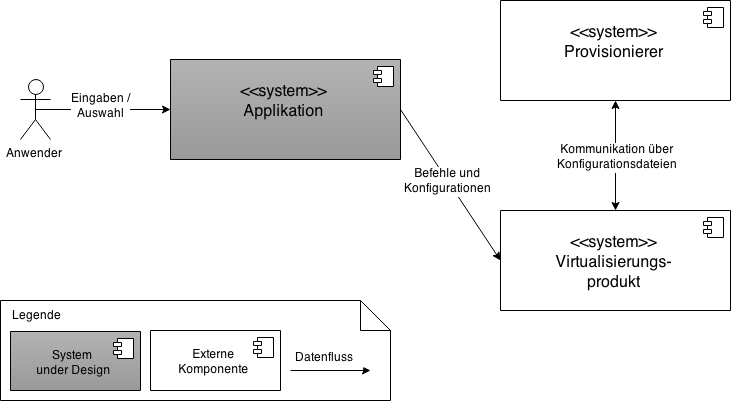
\includegraphics[scale=0.5]{../Bilder/kontextsicht.png}
	\captionof{figure}[kurze Bildunterschrift]{Bildunterschrift}
 \end{minipage}
\end{center}

\subsubsection{Kurzbeschreibung der externen Schnittstellen}
\begin{tabular}{p{4cm} p{10cm}}
\textbf{Eingaben / Auswahl} & Der Awender t�tigt Eingaben und w�hlt unter Optionen aus, die von der Anwendung bereitgestellt werden. Diese werden direkt von der Applikation verarbeitet\\
\textbf{Befehle und Konfigurationen} & Die Applikation erstellt n�tige Konfigurationsdateien und leitet Befehle f�r das Virtualisierungsprodukt weiter\\
\textbf{Kommunikation �ber Konfigurationsdateien} & Das Virtualisierungsproduk ruft �ber die erstellen Konfigurationsdateien auf den Provisionierer zu. \textbf{[TODO MUSS NOCH BEARBEITET WERDEN]}.
\end{tabular}



\chapter{Sichten}
\section{Bausteinsicht}
\section{Laufzeitsicht}
\section{Verteilungssicht}
\section{Zusammenfassung}
